\documentclass{beamer}
\usetheme{CambridgeUS}

\usepackage{svg}
\usepackage{xcolor}
\usepackage{ragged2e}
\usepackage{minted}
\usepackage{tikz}
\usetikzlibrary{
    backgrounds,
    automata,
    positioning
}

\tikzset{
    ->,
    >=stealth,
    node distance=1.3cm,
    every state/.style={thick, fill=gray!10},
    initial text=,
}%

\title{COD2LEX}
\subtitle{Analisador Léxico Web App}
\author{Pablo Cecilio}
\date{\today}
\titlegraphic{\includegraphics[width=0.4\textwidth]{img/logo_ufsj02.png}}

\begin{document}

\begin{frame}
    \titlepage 
\end{frame}

\section{Introdução}
\begin{frame}{\raisebox{-0.2\height}{\includesvg[width=0.5cm]{img/code-square}}~Introdução}

\end{frame}

\section{Estrutura de Dados}
\begin{frame}[fragile]{\raisebox{-0.2\height}{\includesvg[width=0.5cm]{img/code-square}}~Implementação}
\vspace{-10mm}
\begin{columns}[t]
\begin{column}{0.45\textwidth}
   \begin{figure}
      \centering
      \resizebox{.9\linewidth}{!}{%
      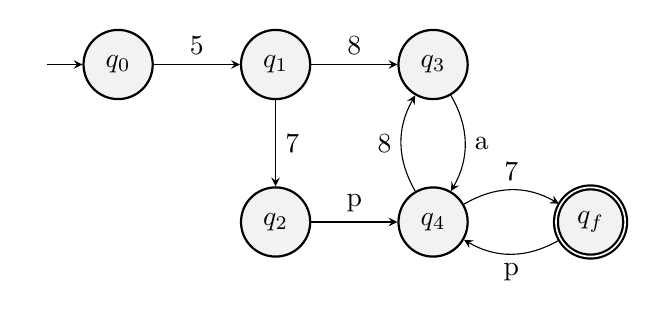
\begin{tikzpicture}[node distance=2cm,on grid,auto]
       \node[state,initial] (q_0) {$q_0$}; 
       \node[state] (q_1) [right of=q_0] {$q_1$};
       \node[state] (q_2) [below of=q_1] {$q_2$};
       \node[state] (q_3) [right of=q_1] {$q_3$};
       \node[state] (q_4) [below of=q_3] {$q_4$};
       \node[state,accepting] (q_5) [right of=q_4] {$q_f$};
        \path
        (q_0) edge node {5} (q_1)
        (q_1) edge node {8} (q_3)
        (q_1) edge node {7} (q_2)
        (q_2) edge node {p} (q_4)
        (q_3) edge[bend left, right] node {a} (q_4)
        (q_4) edge[bend left, left] node {8} (q_3)
        (q_4) edge[bend left, above] node {7} (q_5)
        (q_5) edge[bend left, below] node {p} (q_4);
      \end{tikzpicture}}
      \caption{ER = 5(7p+8a)*7}
    \end{figure}
    \small \justifying Uma maneira simples de implementar um AFD é com um dicionário de dicionários. Cada estado possui um dicionário com suas chaves definidas por suas transições, e os valores de cada chave definem o estado dessa transição.
\end{column}
\begin{column}{0.45\textwidth}
\begin{minted}[fontsize=\footnotesize]{python}
AFD = {
    0:{'5':1},
    1:{'7':2, '8':3},
    2:{'p':4},
    3:{'a':4},
    4:{'8':3, '7':5},
    5:{'p':4}
    }
estado = 0
final = {5}
for c in str:
    try:
        estado = AFD[estado][c]
    except KeyError:
        break
if estado in final:
    print('Entrada Aceita.')
\end{minted}
\end{column}
\end{columns}
\end{frame}

\section{Estrutura de Dados}
\begin{frame}[fragile]{\raisebox{-0.2\height}{\includesvg[width=0.5cm]{img/code-square}}~Implementação pela Tabela de Transição}

\begin{columns}
\begin{column}{0.45\textwidth}
    \small \justifying Utilizando o mesmo principio porem com uma logica diferente, o mesmo automato pode ser implementado por meio de sua tabela de transição.
    
    \begin{block}{get\_transition()}
    \small Esta função retorna o índice da coluna na tabela de transições; expressões regulares podem ser usadas na validação.
    \end{block}
    
\end{column}
\begin{column}{0.45\textwidth}
\begin{minted}[fontsize=\scriptsize]{python}
tabelaTR = {
          #  5   7   p   8   a  [.]
     "0": [  1, -1, -1, -1, -1, -1],
     "1": [ -1,  2, -1,  3, -1, -1],
     "2": [ -1, -1,  4, -1, -1, -1],
     "3": [ -1, -1, -1, -1,  4, -1],
     "4": [ -1,  5, -1,  3, -1, -1],
     "5": [ -1,  4, -1, -1, -1, -1]
    }
estado = 0
final = {5}
for c in str:
    tr = get_transition(c)
    estado = tabelaTR[str(estado)][tr]
    if estado == -1:
        break
if estado in final:
    print('Entrada Aceita.')
\end{minted}
\end{column}
\end{columns}
\end{frame}

\end{document}